\documentclass{HZNUMCM}
\usepackage{graphicx}
\usepackage{hyperref}
\usepackage{subcaption}
\definecolor{customcolor}{HTML}{429938}

\setControlNumber{888888}
\setContestType{MCM}
\setProblemLetter{A}
\setPaperTitle{Our Article}

%summary
\setSummary{ sumary sumary sumary sumary sumary sumary sumary sumary sumary sumary sumary sumary sumary sumary sumary sumary sumary sumary sumary sumary sumary sumary sumary sumary sumary sumary sumary sumary sumary sumary sumary sumary sumary sumary sumary sumary sumary sumary sumary sumary sumary sumary sumary sumary sumary sumary sumary sumary sumary sumary sumary sumary sumary sumary sumary sumary sumary sumary sumary sumary sumary sumary sumary sumary sumary sumary sumary sumary sumary sumary sumary sumary sumary sumary sumary sumary sumary sumary sumary sumary sumary sumary sumary sumary sumary sumary sumary sumary sumary sumary sumary sumary sumary sumary sumary sumary sumary sumary sumary sumary sumary sumary sumary sumary sumary sumary sumary sumary sumary sumary sumary sumary sumary sumary sumary sumary sumary sumary sumary sumary sumary sumary sumary sumary sumary sumary sumary sumary sumary sumary sumary sumary sumary sumary sumary sumary sumary sumary sumary sumary sumary sumary sumary sumary sumary sumary sumary sumary sumary sumary sumary sumary sumary sumary sumary sumary sumary sumary sumary sumary sumary sumary sumary sumary sumary sumary sumary sumary sumary sumary sumary sumary sumary sumary sumary sumary sumary sumary sumary sumary sumary sumary sumary sumary sumary sumary sumary sumary sumary sumary sumary sumary sumary sumary sumary sumary sumary sumary sumary sumary sumary sumary sumary sumary sumary sumary sumary sumary sumary sumary sumary sumary sumary sumary sumary sumary sumary sumary sumary sumary sumary sumary sumary sumary sumary sumary sumary sumary sumary sumary sumary sumary sumary sumary sumary sumary sumary sumary sumary sumary sumary sumary sumary sumary sumary sumary sumary sumary sumary sumary sumary sumary sumary sumary sumary sumary sumary sumary sumary sumary sumary sumary sumary sumary sumary sumary sumary sumary sumary sumary sumary sumary sumary sumary sumary sumary sumary sumary sumary sumary sumary sumary sumary sumary sumary sumary sumary sumary sumary sumary sumary sumary sumary sumary sumary sumary sumary sumary sumary sumary sumary sumary sumary sumary sumary sumary sumary sumary sumary sumary sumary sumary sumary sumary sumary sumary sumary sumary sumary}

%begin
\begin{document}
\showSummarySheet
\showContents

  \section{Introduction}
    \subsection{Background}
    \subsection{Problem Analysis}
    \subsection{Our Work}
    \begin{itemize}
      \item 1
      \item 2
      \item 3
    \end{itemize}

  \section{Assumptions and Notations}
    \subsection{Assumptions and Explanation}
      \begin{itemize}
        \item \textbf{Geographic Applicability Assumption}: The model assumes that the applicable region is Southeast Asia.

        \textbf{Explanation}: The climate of Southeast Asia is simple, with only two seasons—rainy and dry. Additionally, the temperature variation within a year is minimal.
        \item \textbf{Planting Pattern Assumption}: The model assumes that two crops of rice are planted each year in the farmland.
  
        \textbf{Explanation}: This aligns with the planting patterns commonly observed in Southeast Asia, and the simplicity of crop types makes the model easier to establish.
        \item \textbf{Stable Growth Environment Assumption}: The model assumes that no natural disasters, which could significantly impact the agricultural ecosystem, will occur during the time frame considered.
  
        \textbf{Explanation}: Natural disasters are considered low-probability events in agricultural activities. To ensure the generalizability of the model, natural disasters should not be considered.
      \end{itemize}
        \subsection{Notations}
      % table
      \begin{table}[h]
        \centering
        % \caption{An example of a three-line table.}
        \begin{tabular}{cc}
          \toprule
          \rowcolor{customcolor!40} % 设置背景颜色
          Symbols & Description\\
          \midrule
          $\mathbf{X}$ & Vector $[N_w,N_c,N_p,N_b,N_B,C_{hc},C_{pc}]^T$,etc. \\
          $w$ & Subscription for weeds \\
          $c$ & Subscription for crops \\
          $p$ & Subscription for pest \\
          $bir$ & Subscription for birds \\
          $bat$ & Subscription for bats \\
          $hc$ & Subscription for herbicide \\
          $pc$ & Subscription for pesticide \\
          $C_i$ & Concentration of certain chemical \\
          $N_i$ & Numbers of certain species \\
          $\alpha$ & $abc$ \\
          \bottomrule
        \end{tabular}
        \label{tab:example}
      \end{table}

  \section{Models}

  \section{Application of the Models}

  \section{Sensitivity Analysis}

  \section{Evaluation of the Model}
    \subsection{Strengths}
    \subsection{Weaknesses}

  \section{Conclusion}

  % % figure
  % \begin{figure}[ht]
  %   \centering
  %   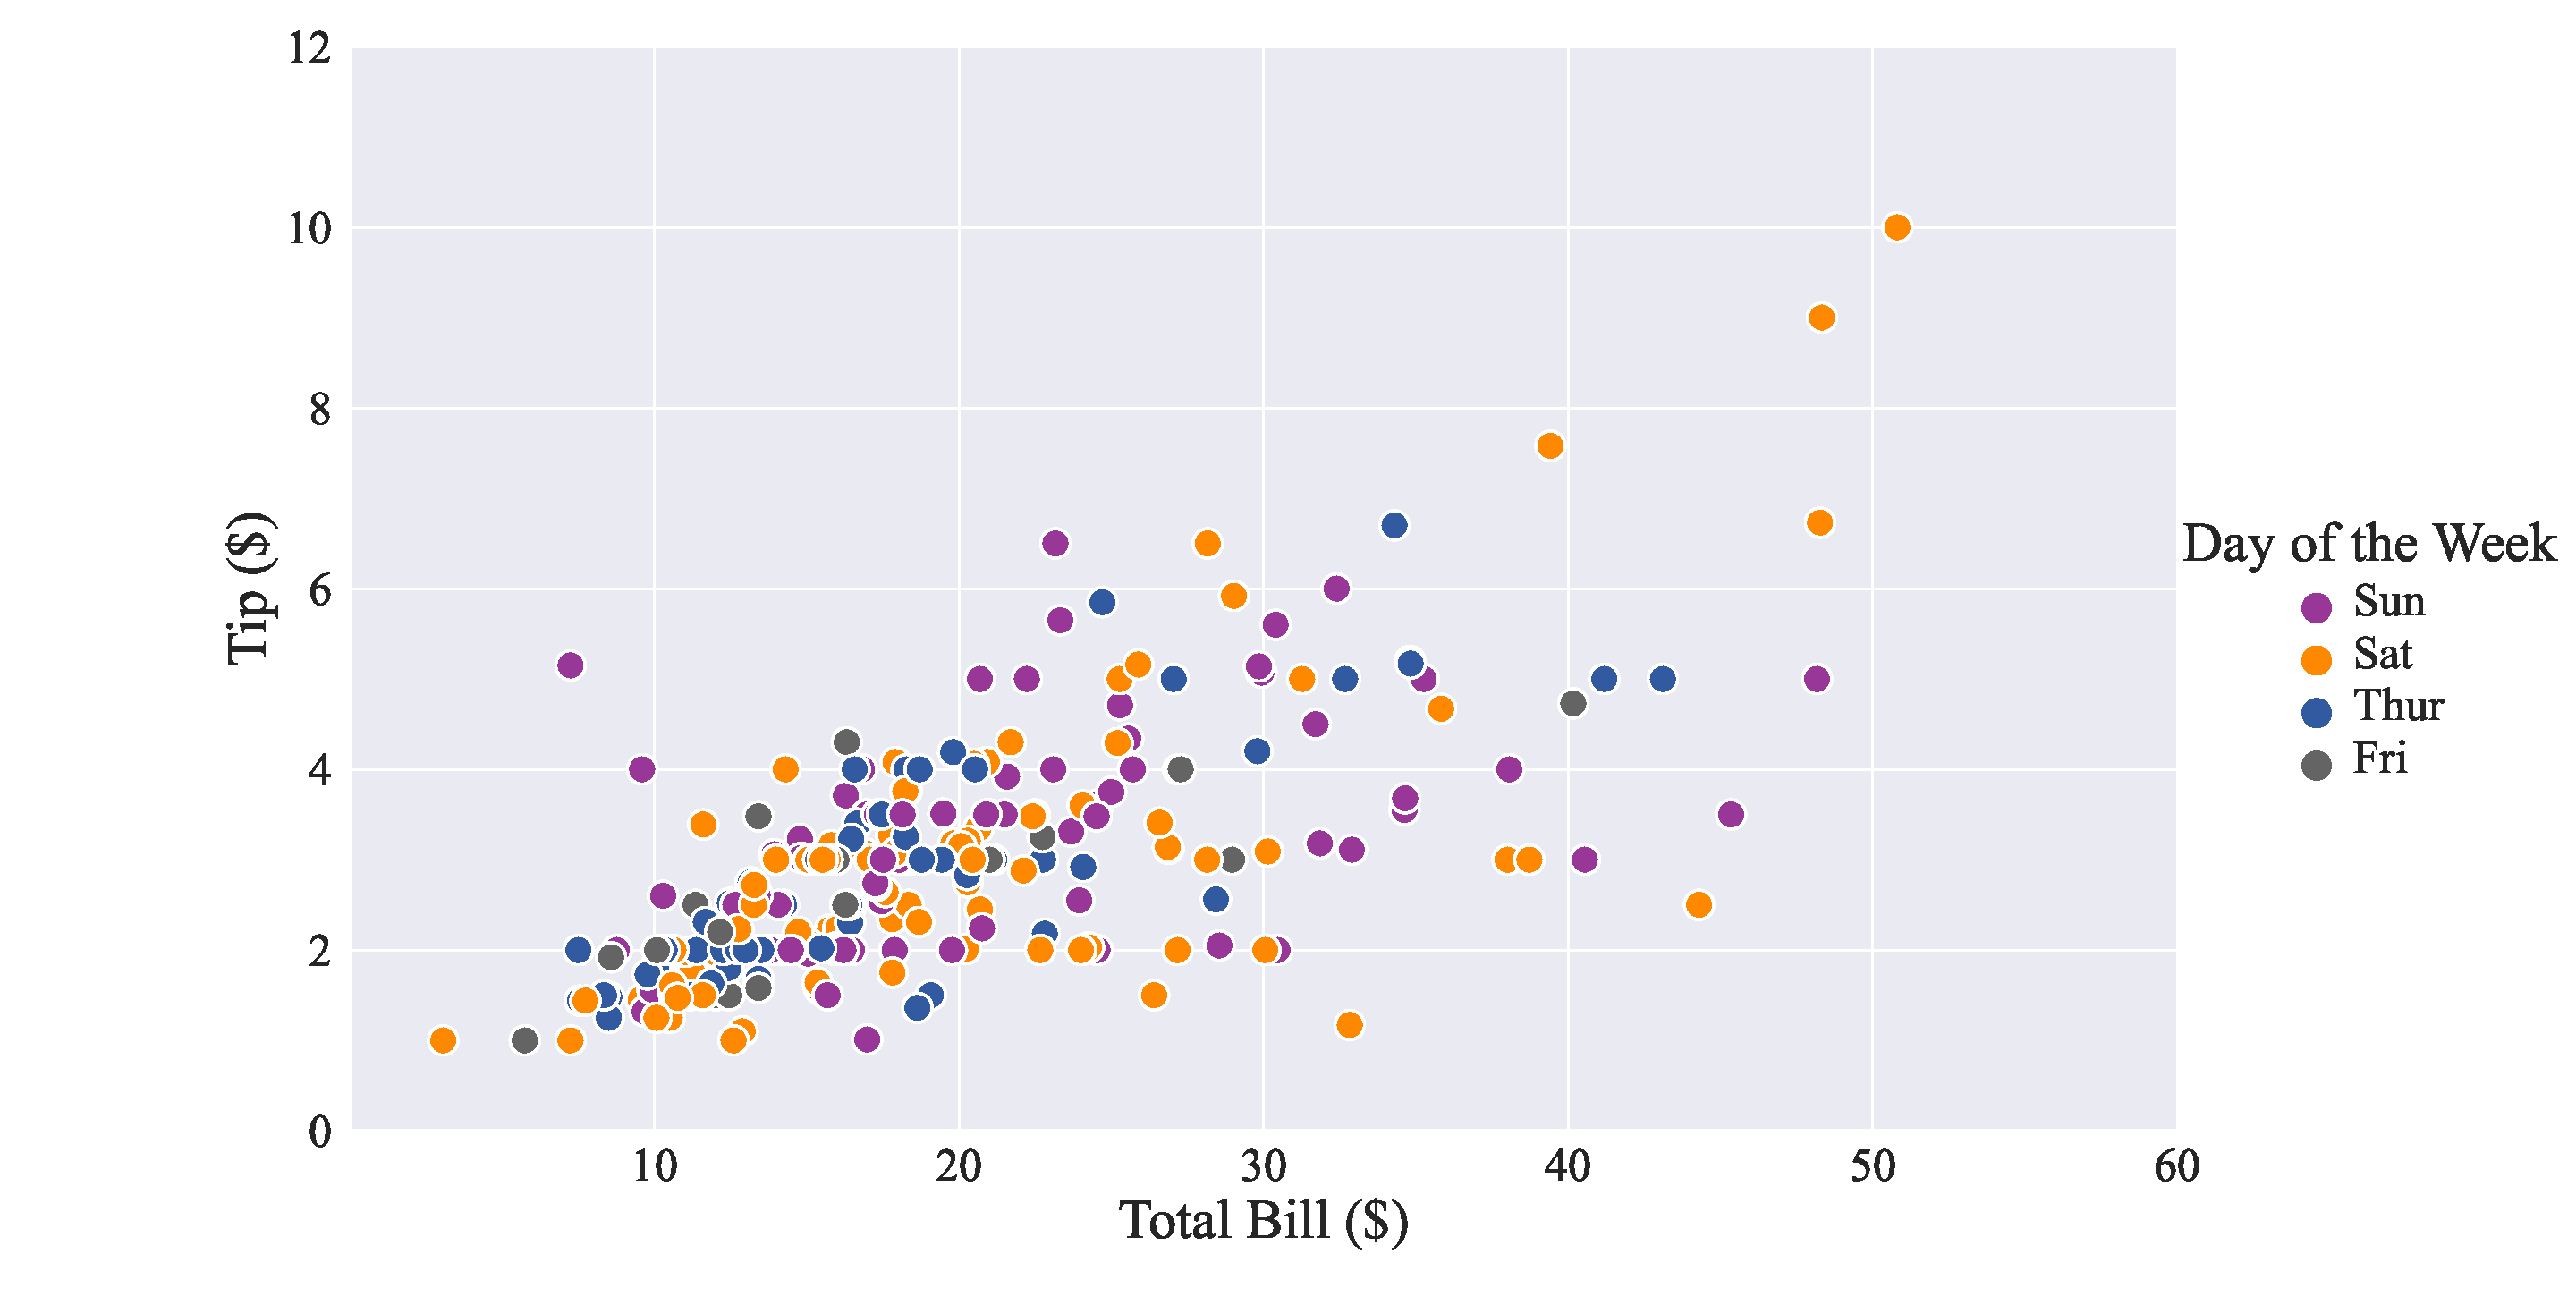
\includegraphics[width=\linewidth]{images/scatter.pdf} % 替换为你的第一张图片路径
  %   \caption{the scatter}
  %   \label{fig:image1}
  % \end{figure}

  % \begin{figure}[ht]
  %     \centering
  %     \begin{minipage}[b]{0.45\linewidth}
  %         \centering
  %         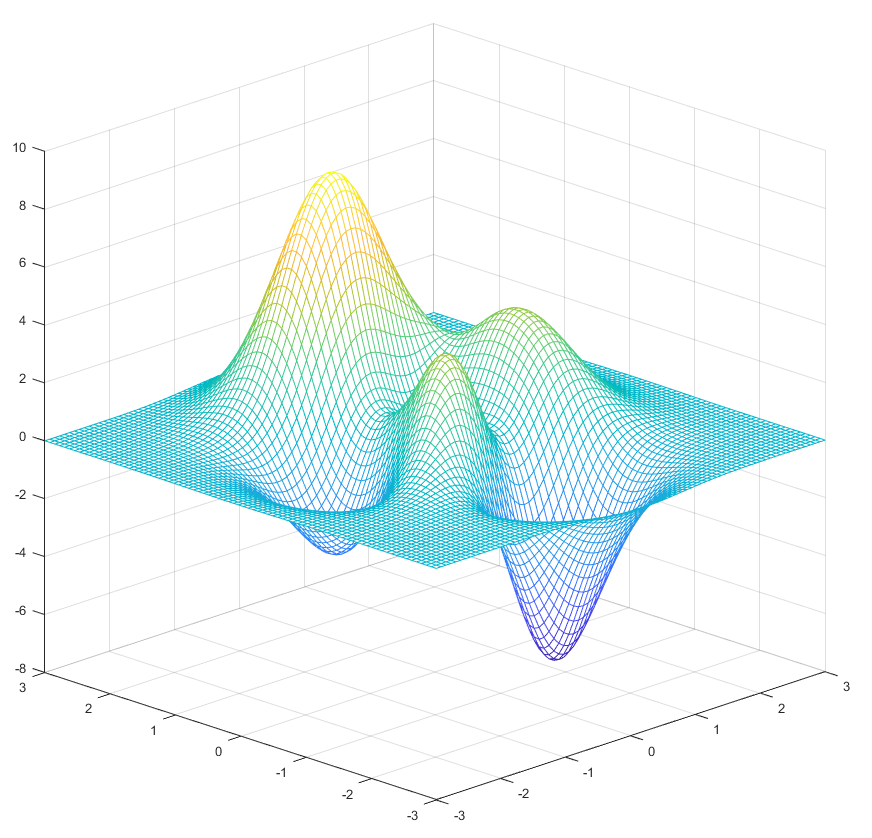
\includegraphics[height=5cm, keepaspectratio]{images/peaks.png} % 替换为你的第一张图片路径
  %         \caption{First Image}
  %         \label{fig:image2}
  %     \end{minipage}
  %     \hspace{0.05\linewidth}
  %     \begin{minipage}[b]{0.45\linewidth}
  %         \centering
  %         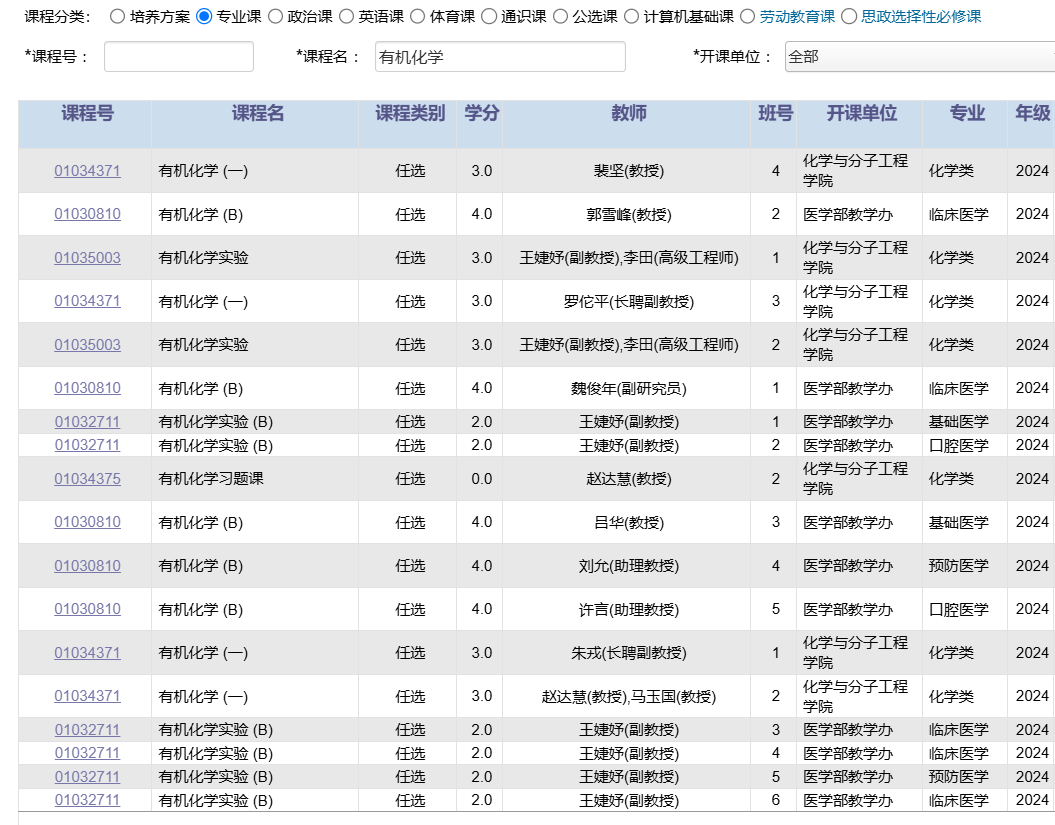
\includegraphics[height=5cm, keepaspectratio]{images/courses.png} % 替换为你的第二张图片路径
  %         \caption{Second Image}
  %         \label{fig:image3}
  %     \end{minipage}
  % \end{figure}

  %%citation
  % as \figurename~\ref{fig:image1} shows,this is a picture.
  % ...\cite{example1}
  % 123123123\cite{rosenow1983drought}

  % % table
  % \begin{table}[h]
  %   \centering
  %   \caption{An example of a three-line table.}
  %   \begin{tabular}{lccc}
  %     \toprule
  %     \rowcolor{customcolor!50} % 设置背景颜色
  %     Column 1 & Column 2 & Column 3 & Column 4 \\
  %     \midrule
  %     Data 1 & Data 2 & Data 3 & Data 4 \\
  %     Data 4 & Data 5 & Data 6 & Data 8 \\
  %     \bottomrule
  %   \end{tabular}
  %   \label{tab:example}
  % \end{table}

  \addcontentsline{toc}{section}{References}
  \bibliographystyle{unsrt}%{brief}%{alpha}%{unsrt}
  \bibliography{article_file}

\end{document}